\documentclass{beamer}
\usepackage[orientation=landscape, size=a0, scale = 1.25]{beamerposter}
\usepackage{graphicx}  % Required for including images
\usepackage{booktabs} % Top and bottom rules for tables
\usepackage{subcaption}
\usepackage{tcolorbox}
\usepackage{tikz}
\usetikzlibrary{shapes, shapes.geometric, shapes.symbols,
shapes.arrows}
\usepackage{epstopdf}
\setlength{\leftmargini}{5cm}

\usetheme{confposter} 
        
\newlength{\sepwid}
\newlength{\onecolwid} 
\newlength{\twocolwid}
\newlength{\threecolwid}
\setlength{\sepwid}{0.024\paperwidth} % Separation width (white space) between columns
\setlength{\onecolwid}{0.3\paperwidth} % Width of one column
\setlength{\twocolwid}{0.464\paperwidth} % Width of two columns
\setlength{\threecolwid}{0.708\paperwidth} % Width of three columns
\setlength{\topmargin}{-0.5in} % Reduce the top margin size
 
\title{Data-Driven Lightweight Encoding Selection} 
\author{Hao Jiang, Aaron J. Elmore} % Author(s)
\institute{Department of Computer Science\\ The University of Chicago} %
\date{}

\tcbset{fonttitle=\bfseries,toptitle=5mm, bottomtitle=5mm}

% Institution(s)    
\addtobeamertemplate{headline}{} 
{
\begin{tikzpicture}[remember picture,overlay] 
\node [shift={(10cm,-3.5cm)}] at (current page.north west)
{
\includegraphics[scale=0.5]{./img/logo_rgb_maroon}};
\node [shift={(9cm,-9cm)}] at (current page.north west)
{
\includegraphics[scale=0.3]{./img/ceres-logo}};
\end{tikzpicture}  
}
\begin{document}

\begin{frame}[t] % The whole poster is enclosed in one beamer frame
 
\usebeamerfont{block body}
\begin{beamercolorbox}[colsep*=2ex,vmode]{block body}
\leftskip4cm
\rightskip4cm

This project explores an automated method to select efficient lightweight
encoding schemes for column-based databases. Existing
methods either rely on database administrators' experience or use simple rules
to make selection. In practice, neither of these methods achieve optimal
performance. We propose a method to solve the problem in a systematic
data-driven way.
 

\end{beamercolorbox}

\begin{columns}[t] 
% The whole poster consists of three major columns, the second of which is
% split into two columns twice - the [t] option aligns each column's content to the top
\begin{column}{\sepwid}\end{column} % Empty spacer column

\begin{column}{\onecolwid} % The first column
          
\begin{block}{Lightweight Encoding}
Popular Lightweight encoding schemes includes Run-Length Encoding, Dictionary
Encoding, Bit-Packing and Delta Encoding. Comparing to popular compression
techniques like gzip and snappy, lightweight encoding schemes have many
advantanges such as Encoding Speed, Local Computation and Support to In-Site
Query Execution.

Best encoding scheme given a data attributes is determined by many
factors including data type and data nature, and there is no simple rule on
how to choose it. The system we propose includes the following features:
\begin{enumerate}\setlength{\itemindent}{1.5em}
  \item Dataset Analysis
  \item Pattern Mining
  \item Data-Driven Encoding Prediction
\end{enumerate}
\end{block}


\begin{block}{Dataset Analysis}
We have collected over 7000 columns from approximately 1200 datasets
with a total size of 500G data. These datasets are all from real-world data
sources and cover a rich collection of data types (integer, date, address,
etc.), with diverse data distributions.
\begin{figure}
\begin{subfigure}{0.45\textwidth}
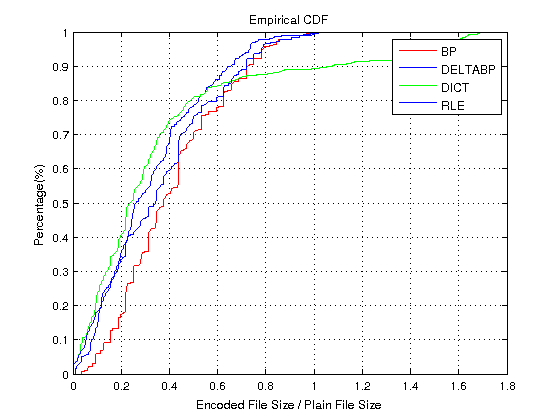
\includegraphics[scale=1]{img/integer_cdf}
\caption{Encoding Compression Ratio for Integer Columns}
\end{subfigure}~
\begin{subfigure}{0.45\textwidth}
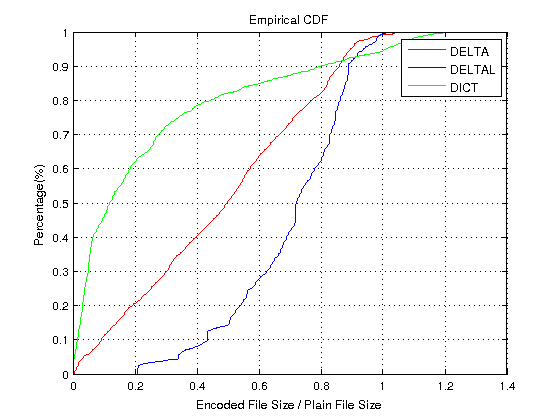
\includegraphics[scale=1]{img/string_cdf}  
\caption{Encoding Compression Ratio for String Columns}
\end{subfigure}
\end{figure}

The figures above show the CDF of the compression ratio for different types of
encodings. It can be seen there is no single best encoding for either data
types.

\end{block}

\end{column}

\begin{column}{\sepwid}\end{column} % Empty spacer column

\begin{column}{\onecolwid} % The second column
\usebeamerfont{block body}
\begin{beamercolorbox}{block body}
Dictionary Encoding is the default encoding for many column storages (e.g,
Apache Parquet and CarbonData). However, the figures below demonstrates that
Dictionary Encoding performs sub-optimal for a considerable amount of data
samples.
\end{beamercolorbox}
\begin{figure}
\begin{subfigure}{0.45\textwidth}
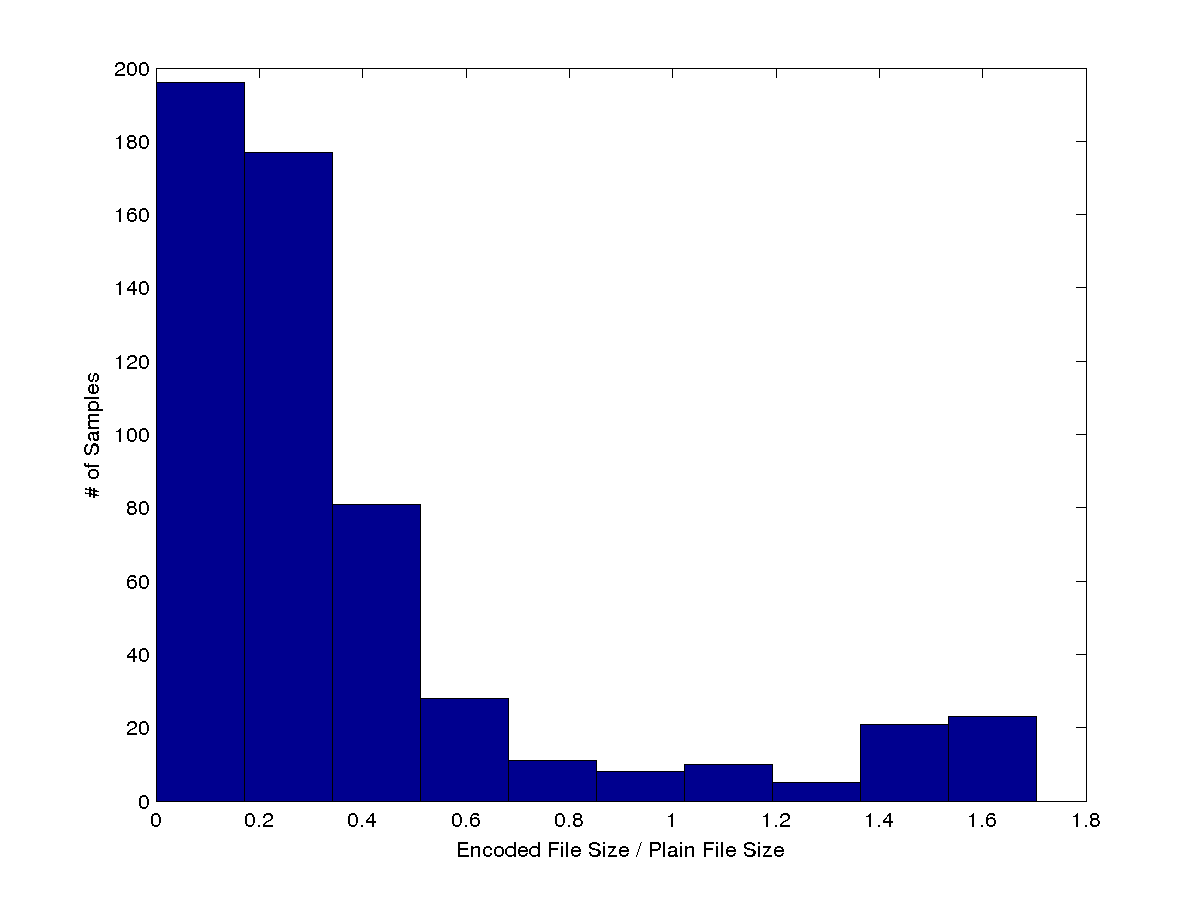
\includegraphics[scale=0.9]{img/integer_dict_hist}
\caption{Dictionary Encoding for Integer Columns}
\end{subfigure}~
\begin{subfigure}{0.45\textwidth}
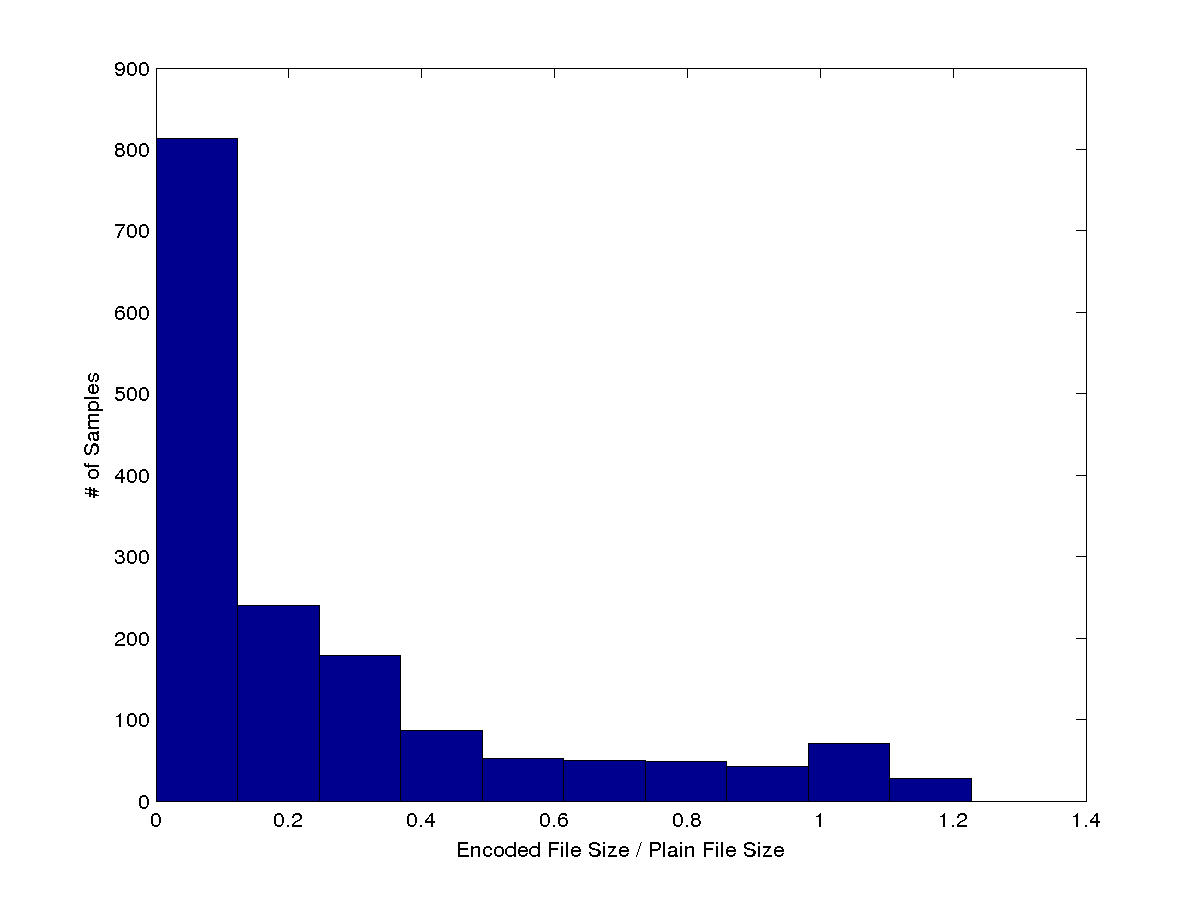
\includegraphics[scale=0.9]{img/string_dict_hist}
\caption{Dictionary Encoding for String Columns}
\end{subfigure}
\end{figure}

\begin{block}{Pattern Mining}
Determining the proper data type is crucial to encoding task. For example,
storing a U.S. phone number in string requires 10 bytes, while storing it in
integer format takes no more than 5 bytes. The challenge is that most real-world
datasets are semi-structured, in which only part of the data contains valid
common structures. We implement multiple Pattern Mining techniques to
automatically identify and extract these structures. 
\vskip0.5cm

\begin{tcolorbox}[colback=green!5!white,colframe=green!60!black,
title=Recognizing Pattern helps better encoding]
\begin{tikzpicture}[]
\normalsize
\node[minimum width = 35cm, minimum height=10cm] at(10,-4) {};
\node[text width=5cm, rounded
corners, fill=green!10,draw=gray!80, inner sep=0.5cm] at (0,-2.5) {
HA32394\\
HB33421\\ 
HA423423\\
HB324234\\
};
\node[text width=8cm] at (0.5,-7) {String format need ~7 Bytes};
\node[single arrow, minimum height=5cm,
draw=gray, fill=orange!30,rotate=25] 
at (7,-1){};
\node[single arrow, minimum height=5cm,
draw=gray, fill=orange!30,rotate=-25] 
at (7,-5){};
\node[text width=4cm, rounded corners, 
fill=green!10,draw=gray!80, inner sep=0.5cm] at (13.5,0) {
HA = 0\\
HB = 1\\ 
HA = 0\\
HB = 1\\
};

\node[text width=8cm] at (21,0) {Categorical Data, 1 bit};

\node[text width=3cm, rounded corners, 
fill=green!10,draw=gray!80, inner sep=0.5cm] at (13,-6) {
32394\\
33421\\ 
23423\\
324234\\
};
\node[text width=9cm] at (21,-6) {Bit-packed Integer, 20 bits};
\end{tikzpicture}

\end{tcolorbox}

In this example, our system observes a pattern <STR><NUM> from the data
column and use this pattern to generate more efficient encoding schemes.

\end{block} 

\end{column}

\begin{column}{\sepwid}\end{column} % Empty spacer olumn

\begin{column}{\onecolwid} % The third column

\begin{tcolorbox}[colback=green!5!white,colframe=green!60!black,
title=Use NLP techniques to discover text patterns]
\begin{tikzpicture}[
marker1/.style={fill=red!30,opacity=0.5,minimum height=1cm},
marker2/.style={fill=blue!30,opacity=0.5,minimum height=1cm},
marker3/.style={fill=blue!30,opacity=0.5,minimum height=1cm}
]
\normalsize

\node[text width=25cm, draw=gray!70, fill=green!20] at (0,0) {
711-2880 Nulla St. Mankato Mississippi 96522\\
P.O. Box 283 8562 Fusce Rd. Frederick Nebraska 20620\\ 
606-3727 Ullamcorper. Street Roseville NH 11523\\
Ap #867-859 Sit Rd. Azusa New York 39531\\
};
\node[marker1,minimum width=5cm] at (2.5,2) {};
\node[marker1,minimum width=4cm] at (7.5,0.8) {};
\node[marker1,minimum width=2cm] at (5.5,-0.5) {};
\node[marker1,minimum width=4cm] at (1.5,-2) {};

\node[marker2,minimum width=2cm] at (-5,2) {};
\node[marker2,minimum width=2cm] at (-1.5,0.8) {};
\node[marker2,minimum width=3cm] at (-1,-0.5) {};
\node[marker2,minimum width=1.5cm] at (-5,-2) {};

\node[single arrow, minimum height=2cm,
draw=gray, fill=orange!30,rotate=-90] 
at (0,-4){};

\node[text width=11cm, draw=gray!70, fill=green!20] at (-7,-8.5) {
711-2880 Nulla\\
P.O. Box 283 8562 Fusce\\ 
606-3727 Ullamcorper.\\
Ap #867-859 Sit\\
};

\node[text width=2.5cm, draw=gray!70, fill=orange!20] at (1,-8.5) {
St.\\
Rd.\\ 
Street\\
Rd.\\
};

\node[text width=4cm, draw=gray!70, fill=green!20] at (5.5,-8.5) {
Mankato\\
Frederick\\ 
Roseville\\
Azusa\\
};

\node[text width=5cm, draw=gray!70, fill=orange!20] at (11.2,-8.5) {
Mississippi\\
Nebraska\\ 
NH\\
New York\\
};

\node[text width=3cm, draw=gray!70, fill=green!20] at (16.5,-8.5) {
96522\\
20620\\ 
11523\\
39531\\
};
\end{tikzpicture}
\end{tcolorbox}

\vskip1em

\usebeamerfont{block body}
\begin{beamercolorbox}{block body}

We also use NLP techniques to look for similar words in text and identify more
subtle patterns. The example above shows that our method is able to discover two
similar word groups from a column storing address information. This allows us
to encode these words more efficently, in addition, it enable us to use these
words to split the text into pieces and do further pattern mining.
\end{beamercolorbox}

\begin{block}{Data Driven Encoding Prediction}
we are building a data-driven encoding selector using neural network that is
able to "predict" the best encoding scheme by looking at only a limited section
of the entire dataset, e.g., the first 1\% of the records.


\begin{tikzpicture}
\node at (-5,0) {
\includegraphics{img/data}};
\node[single arrow,minimum height=1cm,fill=orange!30] at (-1.5,0) {};
\node at (-5,-4) {\normalsize Datasets};
\node at (2,0) {
\includegraphics[scale=0.5]{img/pattern}};
\node at (2,-4) {\normalsize Pattern Mining}; 
\node[single arrow,minimum height=1cm,fill=orange!30] at (6,0) {};
\node at (12,0)
{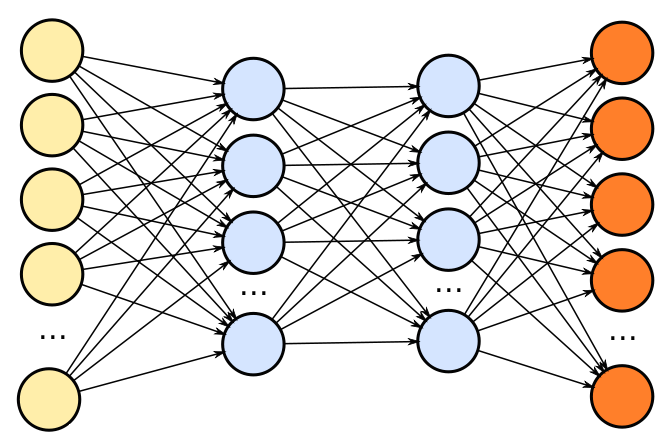
\includegraphics[scale=0.4]{img/deep-neural-network}}; 
\node[text width=10cm] at (12,-4) {\normalsize Prediction Network};
\node at (22,0)
{
\includegraphics[scale=0.15]{img/result}}; 
\node[single arrow,minimum height=1cm,fill=orange!30] at (18,0) {};
\node[text width=10cm] at (23,-4) {\normalsize Efficient Encoding};
\end{tikzpicture}

Choosing core features that truly represents the relationship between data and
label is crucial to the success of neural network training task. The features
we choose including statistical information such as mean and variance of data
length, entropy. We also use NLP technique to learn from column names. Finally,
we also try to use LSTM RNN network to learn patterns from the sampled column.


\end{block}

\end{column}
\begin{column}{\sepwid}\end{column} % Empty spacer column

\end{columns}

\end{frame}
\end{document}